%%%%%%%%%%%%%%%%%%%%%%%%%%%%%%%%%%%%%%%%%
% Beamer Presentation
% LaTeX Template
% Version 1.0 (10/11/12)
%
% This template has been downloaded from:
% http://www.LaTeXTemplates.com
%
% License:
% CC BY-NC-SA 3.0 (http://creativecommons.org/licenses/by-nc-sa/3.0/)
%
%%%%%%%%%%%%%%%%%%%%%%%%%%%%%%%%%%%%%%%%%

%----------------------------------------------------------------------------------------
%	PACKAGES AND THEMES
%----------------------------------------------------------------------------------------

\documentclass{beamer}

\mode<presentation> {

% The Beamer class comes with a number of default slide themes
% which change the colors and layouts of slides. Below this is a list
% of all the themes, uncomment each in turn to see what they look like.

%\usetheme{default}
%\usetheme{AnnArbor}
%\usetheme{Antibes}
%\usetheme{Bergen}
%\usetheme{Berkeley}
%\usetheme{Berlin}
%\usetheme{Boadilla}
%\usetheme{CambridgeUS}
%\usetheme{Copenhagen}
%\usetheme{Darmstadt}
%\usetheme{Dresden}
%\usetheme{Frankfurt}
%\usetheme{Goettingen}
%\usetheme{Hannover}
%\usetheme{Ilmenau}
%\usetheme{JuanLesPins}
%\usetheme{Luebeck}
%\usetheme{Madrid}
%\usetheme{Malmoe}
%\usetheme{Marburg}
%\usetheme{Montpellier}
%\usetheme{PaloAlto}
%\usetheme{Pittsburgh}
%\usetheme{Rochester}
%\usetheme{Singapore}
%\usetheme{Szeged}
\usetheme{Warsaw}

% As well as themes, the Beamer class has a number of color themes
% for any slide theme. Uncomment each of these in turn to see how it
% changes the colors of your current slide theme.

%\usecolortheme{albatross}
%\usecolortheme{beaver}
%\usecolortheme{beetle}
%\usecolortheme{crane}
%\usecolortheme{dolphin}
%\usecolortheme{dove}
%\usecolortheme{fly}
%\usecolortheme{lily}
%\usecolortheme{orchid}
%\usecolortheme{rose}
%\usecolortheme{seagull}
%\usecolortheme{seahorse}
%\usecolortheme{whale}
%\usecolortheme{wolverine}

%\setbeamertemplate{footline} % To remove the footer line in all slides uncomment this line
%\setbeamertemplate{footline}[page number] % To replace the footer line in all slides with a simple slide count uncomment this line

%\setbeamertemplate{navigation symbols}{} % To remove the navigation symbols from the bottom of all slides uncomment this line
}

\usepackage{graphicx} % Allows including images
\usepackage{booktabs} % Allows the use of \toprule, \midrule and \bottomrule in tables

\newcommand\smallfont{\fontsize{8}{7.2}\selectfont}

%----------------------------------------------------------------------------------------
%	TITLE PAGE
%----------------------------------------------------------------------------------------

\title[Cognitive Urban Settlement Model]{A comparison of cognitive vs. Cobb-Douglas decision making in models of residential location selection} % The short title appears at the bottom of every slide, the full title is only on the title page

\author{Vince Kane} % Your name
\institute[George Mason University] % Your institution as it will appear on the bottom of every slide, may be shorthand to save space
{
Computational Social Science Department,\\
George Mason University \\ % Your institution for the title page
\medskip
\textit{vkane2@gmu.edu} % Your email address
}
\date{29 April 2015} % Date, can be changed to a custom date

\begin{document}

\begin{frame}
\titlepage % Print the title page as the first slide
\end{frame}

\begin{frame}
\frametitle{Overview} % Table of contents slide, comment this block out to remove it
\tableofcontents % Throughout your presentation, if you choose to use \section{} and \subsection{} commands, these will automatically be printed on this slide as an overview of your presentation
\end{frame}

%----------------------------------------------------------------------------------------
%	PRESENTATION SLIDES
%----------------------------------------------------------------------------------------

%------------------------------------------------
\section{Introduction} % Sections can be created in order to organize your presentation into discrete blocks, all sections and subsections are automatically printed in the table of contents as an overview of the talk
%------------------------------------------------

\begin{frame}
\frametitle{Cobb-Douglas Utility}

\begin{block}{Cobb-Douglas utility}
\bigskip
$U = {x_1}^{\alpha_1} + {x_2}^{\alpha_2} + ... + {x_N}^{\alpha_N}$
\bigskip
\end{block}

\end{frame}

\section{Method}

\subsection{Base Model (Cobb-Douglas)}

%------------------------------------------------

\begin{frame}
\frametitle{Initialized landscape}

\begin{figure}
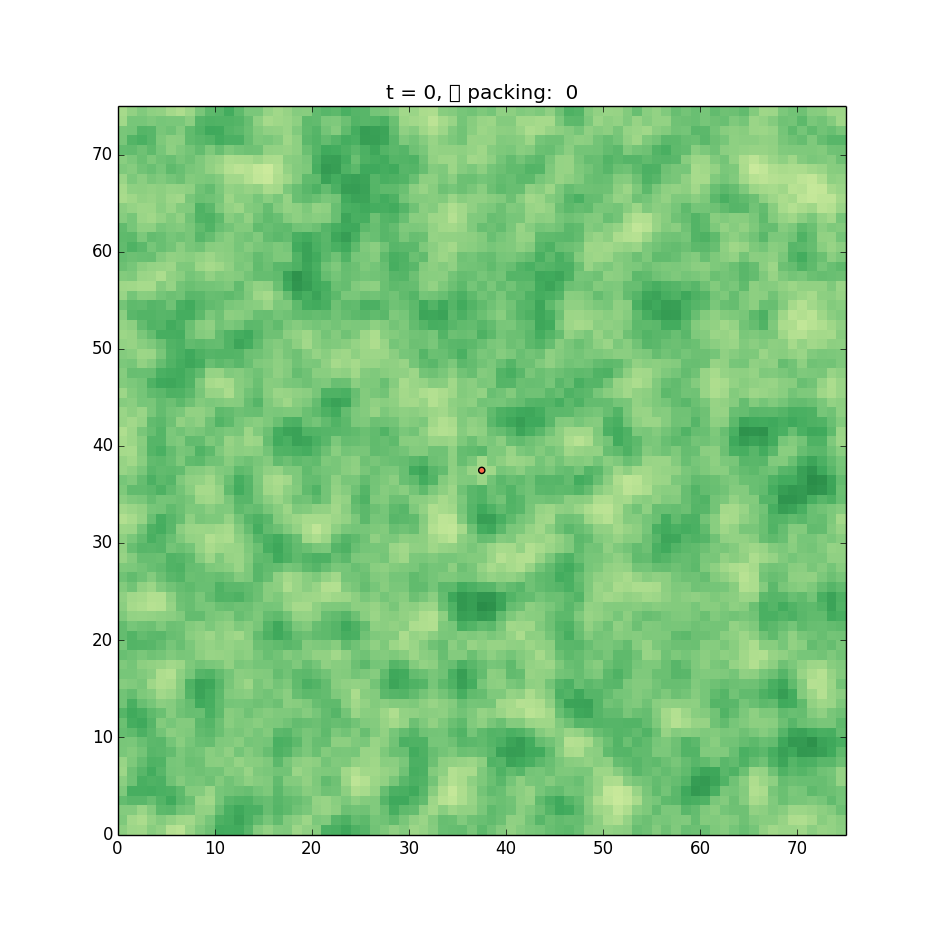
\includegraphics[width=\textwidth,height=0.8\textheight,keepaspectratio]{empty_landscape.png}
\end{figure}

\end{frame}

\subsection{"Take the best"}

%------------------------------------------------

\begin{frame}[fragile] % Need to use the fragile option when verbatim is used in the slide
\frametitle{Decision making code}
\smallfont

\begin{block}{Cobb-Douglas utility maximization}
\begin{verbatim}

        . . .
        
        util = (1/dist)**self.alpha_srv + qual**self.alpha_qua
        choices[eval_patch] = util
    choice = max(list(choices.keys()), key = lambda loc : choices[loc])
    
\end{verbatim}
\end{block}

\begin{block}{"Take the best" approach}
\begin{verbatim}

        . . .
        
        if dist < best_dist and qual > self.alpha_qua*best_qual:
            residence = eval_patch
            best_dist = dist
            best_qual = qual
        if qual > best_qual and dist < (1-self.alpha_srv)*best_dist:
            residence = eval_patch
            best_qual = qual
            best_dist = dist
            
\end{verbatim}
\end{block}

\end{frame}

\section{Results}

\subsection{Qualitative Results}

%------------------------------------------------

\begin{frame}
\frametitle{End run results with maximum preference for quality}

\begin{columns}[t] % The "c" option specifies centered vertical alignment while the "t" option is used for top vertical alignment

\column{.5\textwidth} % Left column and width
\begin{figure}
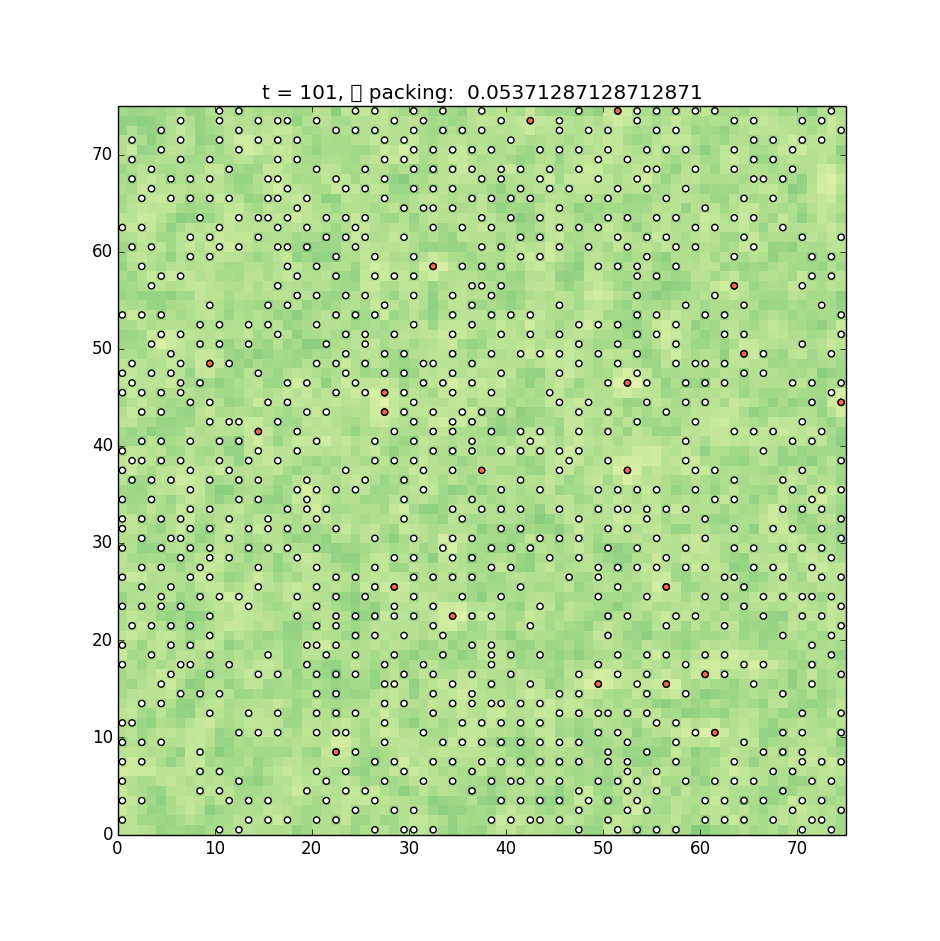
\includegraphics[width=0.9\linewidth]{qual_cd_0_0.png}
\end{figure}
(a) Cobb-Douglas utility maximizers

\column{.5\textwidth} % Right column and width
\begin{figure}
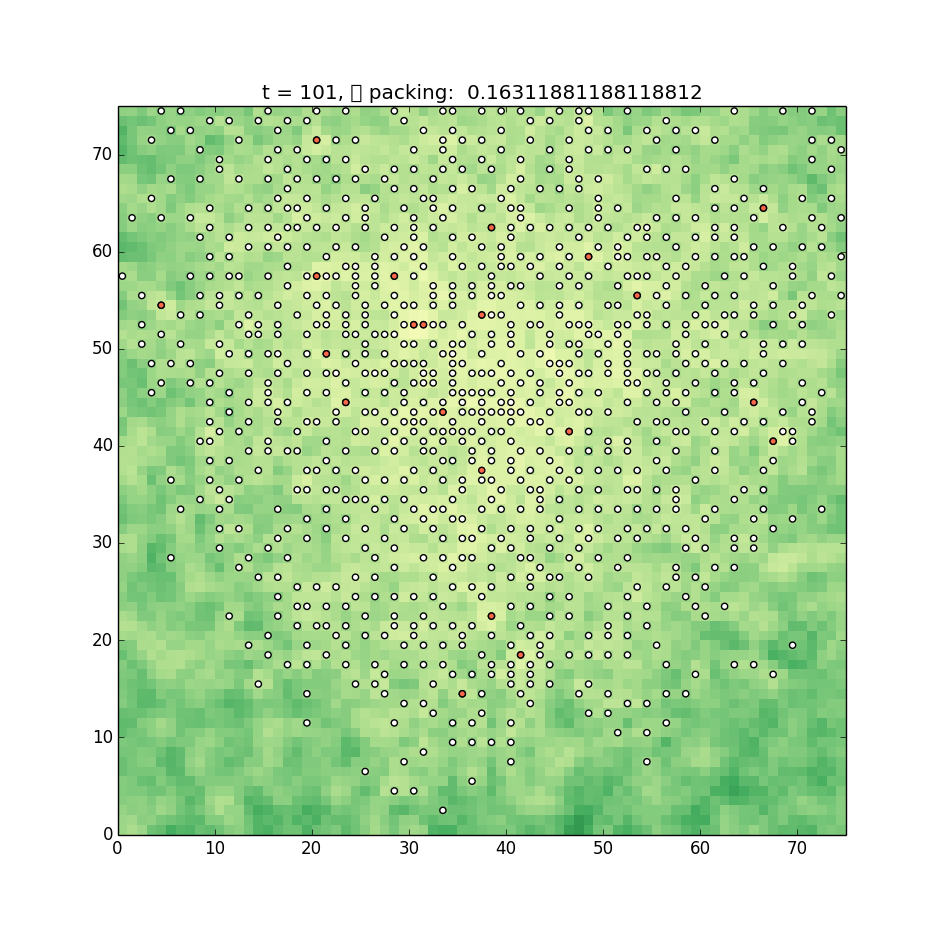
\includegraphics[width=0.9\linewidth]{qual_cog2_0_0.png}
\end{figure}
(b) Cognitive selectors

\end{columns}
\end{frame}

%------------------------------------------------

\begin{frame}
\frametitle{End run results; maximum preference for services proximity}

\begin{columns}[t] % The "c" option specifies centered vertical alignment while the "t" option is used for top vertical alignment

\column{.5\textwidth} % Left column and width
\begin{figure}
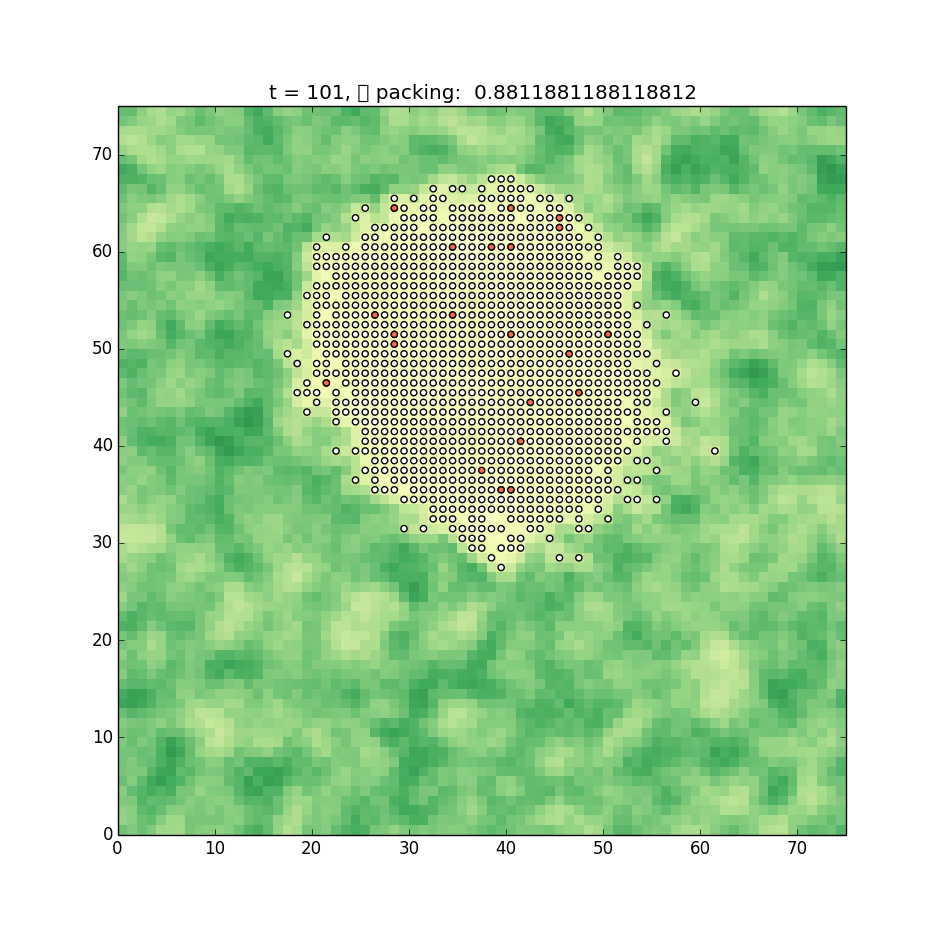
\includegraphics[width=0.9\linewidth]{qual_cd_2_0.png}
\end{figure}
(a) Cobb-Douglas utility maximizers

\column{.5\textwidth} % Right column and width
\begin{figure}
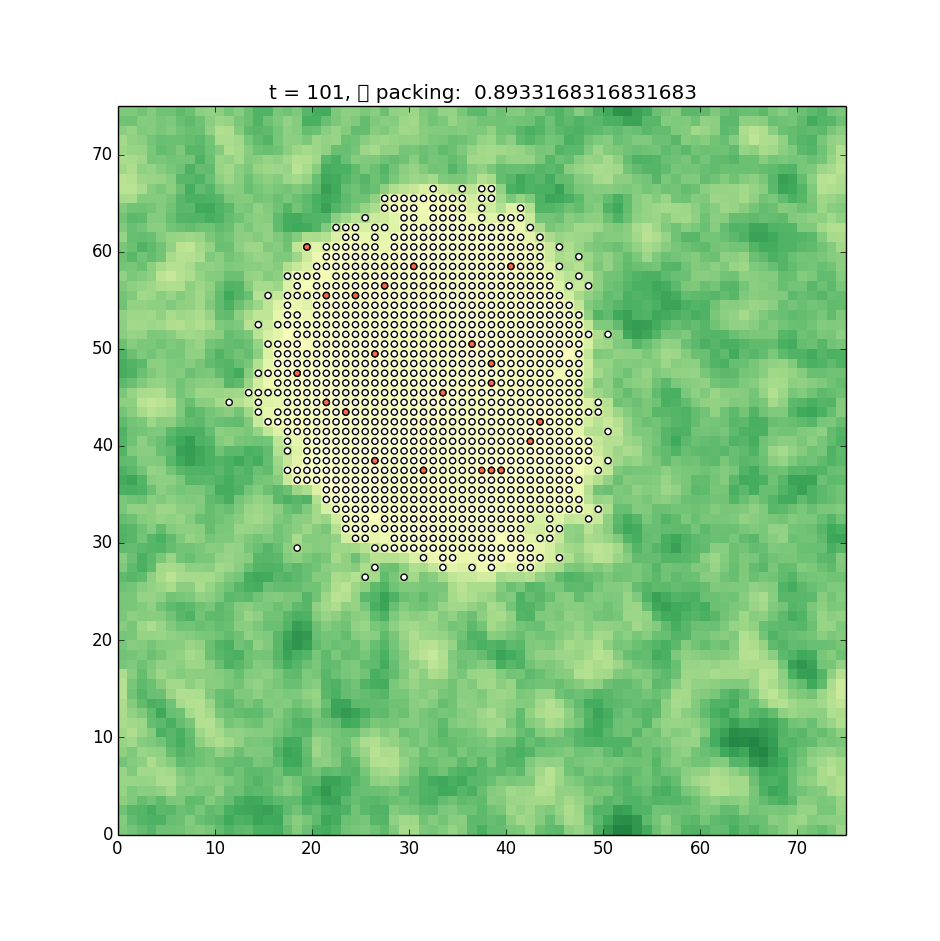
\includegraphics[width=0.9\linewidth]{qual_cog2_2_0.png}
\end{figure}
(b) Cognitive selectors

\end{columns}
\end{frame}

%------------------------------------------------

\begin{frame}
\frametitle{maximum preference for services - cognitive variation}

\begin{columns}[t] % The "c" option specifies centered vertical alignment while the "t" option is used for top vertical alignment

\column{.5\textwidth} % Left column and width
\begin{figure}
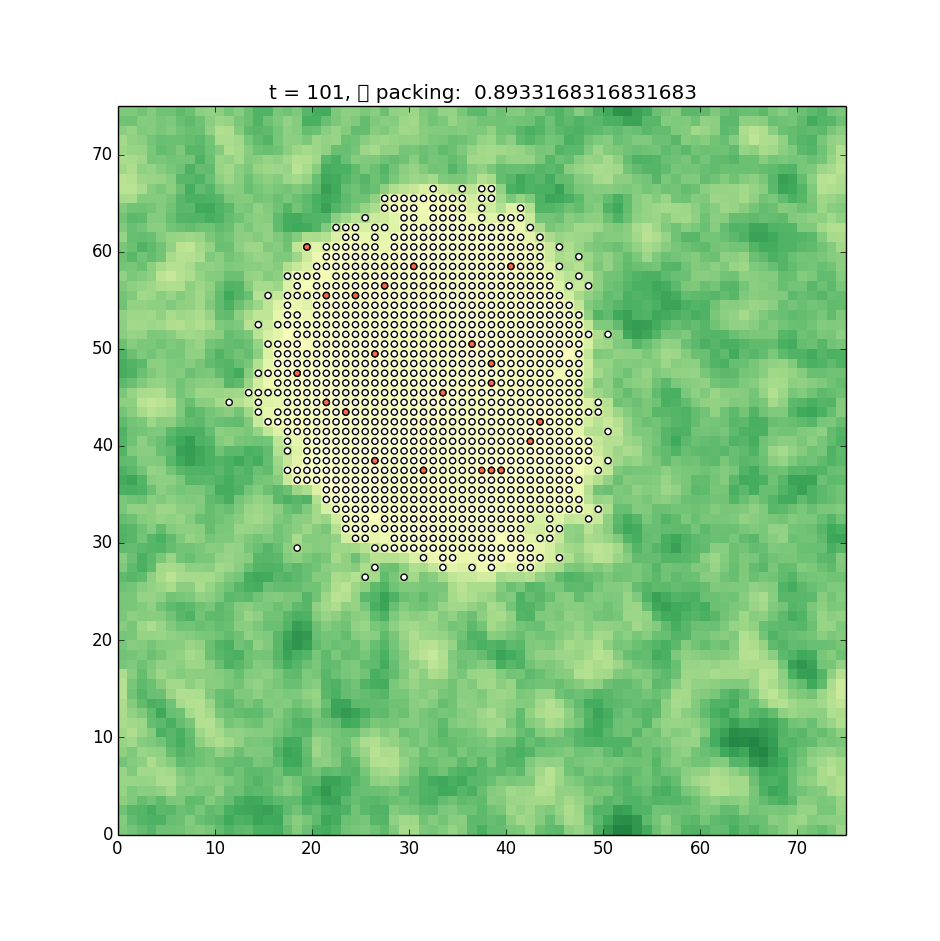
\includegraphics[width=0.9\linewidth]{qual_cog2_2_0.png}
\end{figure}
(a) Cognitive selectors

\column{.5\textwidth} % Right column and width
\begin{figure}
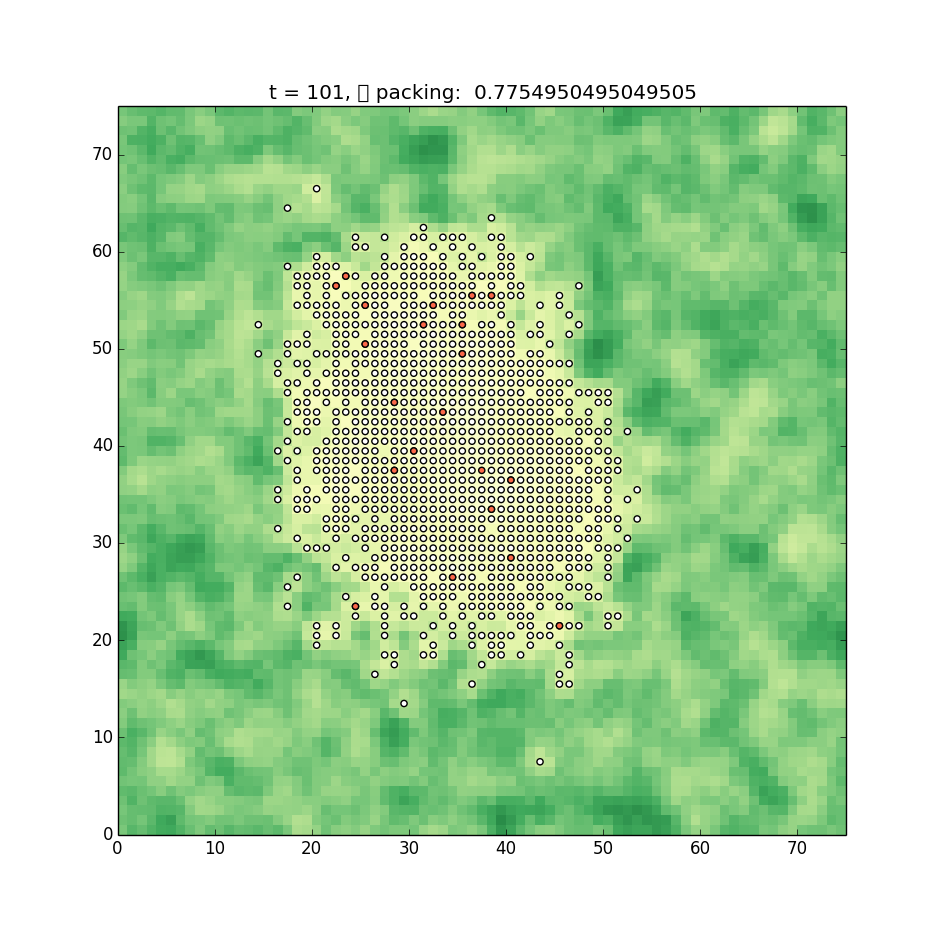
\includegraphics[width=0.9\linewidth]{qual_cog_2_0.png}
\end{figure}
(b) Cognitive selectors, variant

\end{columns}
\end{frame}

\subsection{Quantitative Results}
%------------------------------------------------

\begin{frame}
\frametitle{Parameter sweep results}
Plot of average end run packing fraction vs. preference for services proximity.  Each data point is average of 30 runs to 100 time steps.
\begin{figure}
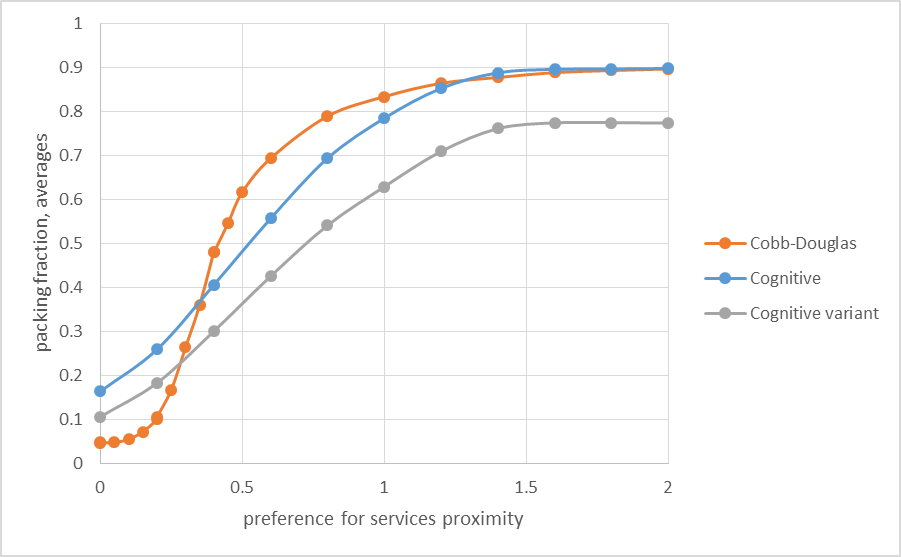
\includegraphics[width=0.8\linewidth]{main_results.png}
\end{figure}
\end{frame}

\section{Discussion and Conclusion}



%------------------------------------------------

\begin{frame}
\Huge{\centerline{The End}}
\end{frame}

%----------------------------------------------------------------------------------------

\end{document} 